\newpage
\section{Project controls}\label{sect:dmpc}

DM follows the Rubin project controls system, as described in \citeds{LPM-98}.
Considerations specific to DM are outlined in \secref{sect:plan}.

The DM Project Controller is responsible for the PMCS and, in particular, for ensuring that DM properly complies with our earned value management requirements.
The Controller is the first point of contact for all questions about the PMCS.

\subsection{Schedule}\label{sect:schedule}

The entire Rubin project schedule is held in Primavera.
Tied to major project milestones we have a series of DM tests which need to be performed to show readiness for the different project phases.
This is depicted in \figref{fig:schedule}.

\begin{figure}[htbp]
	\hspace{-0.5cm}	 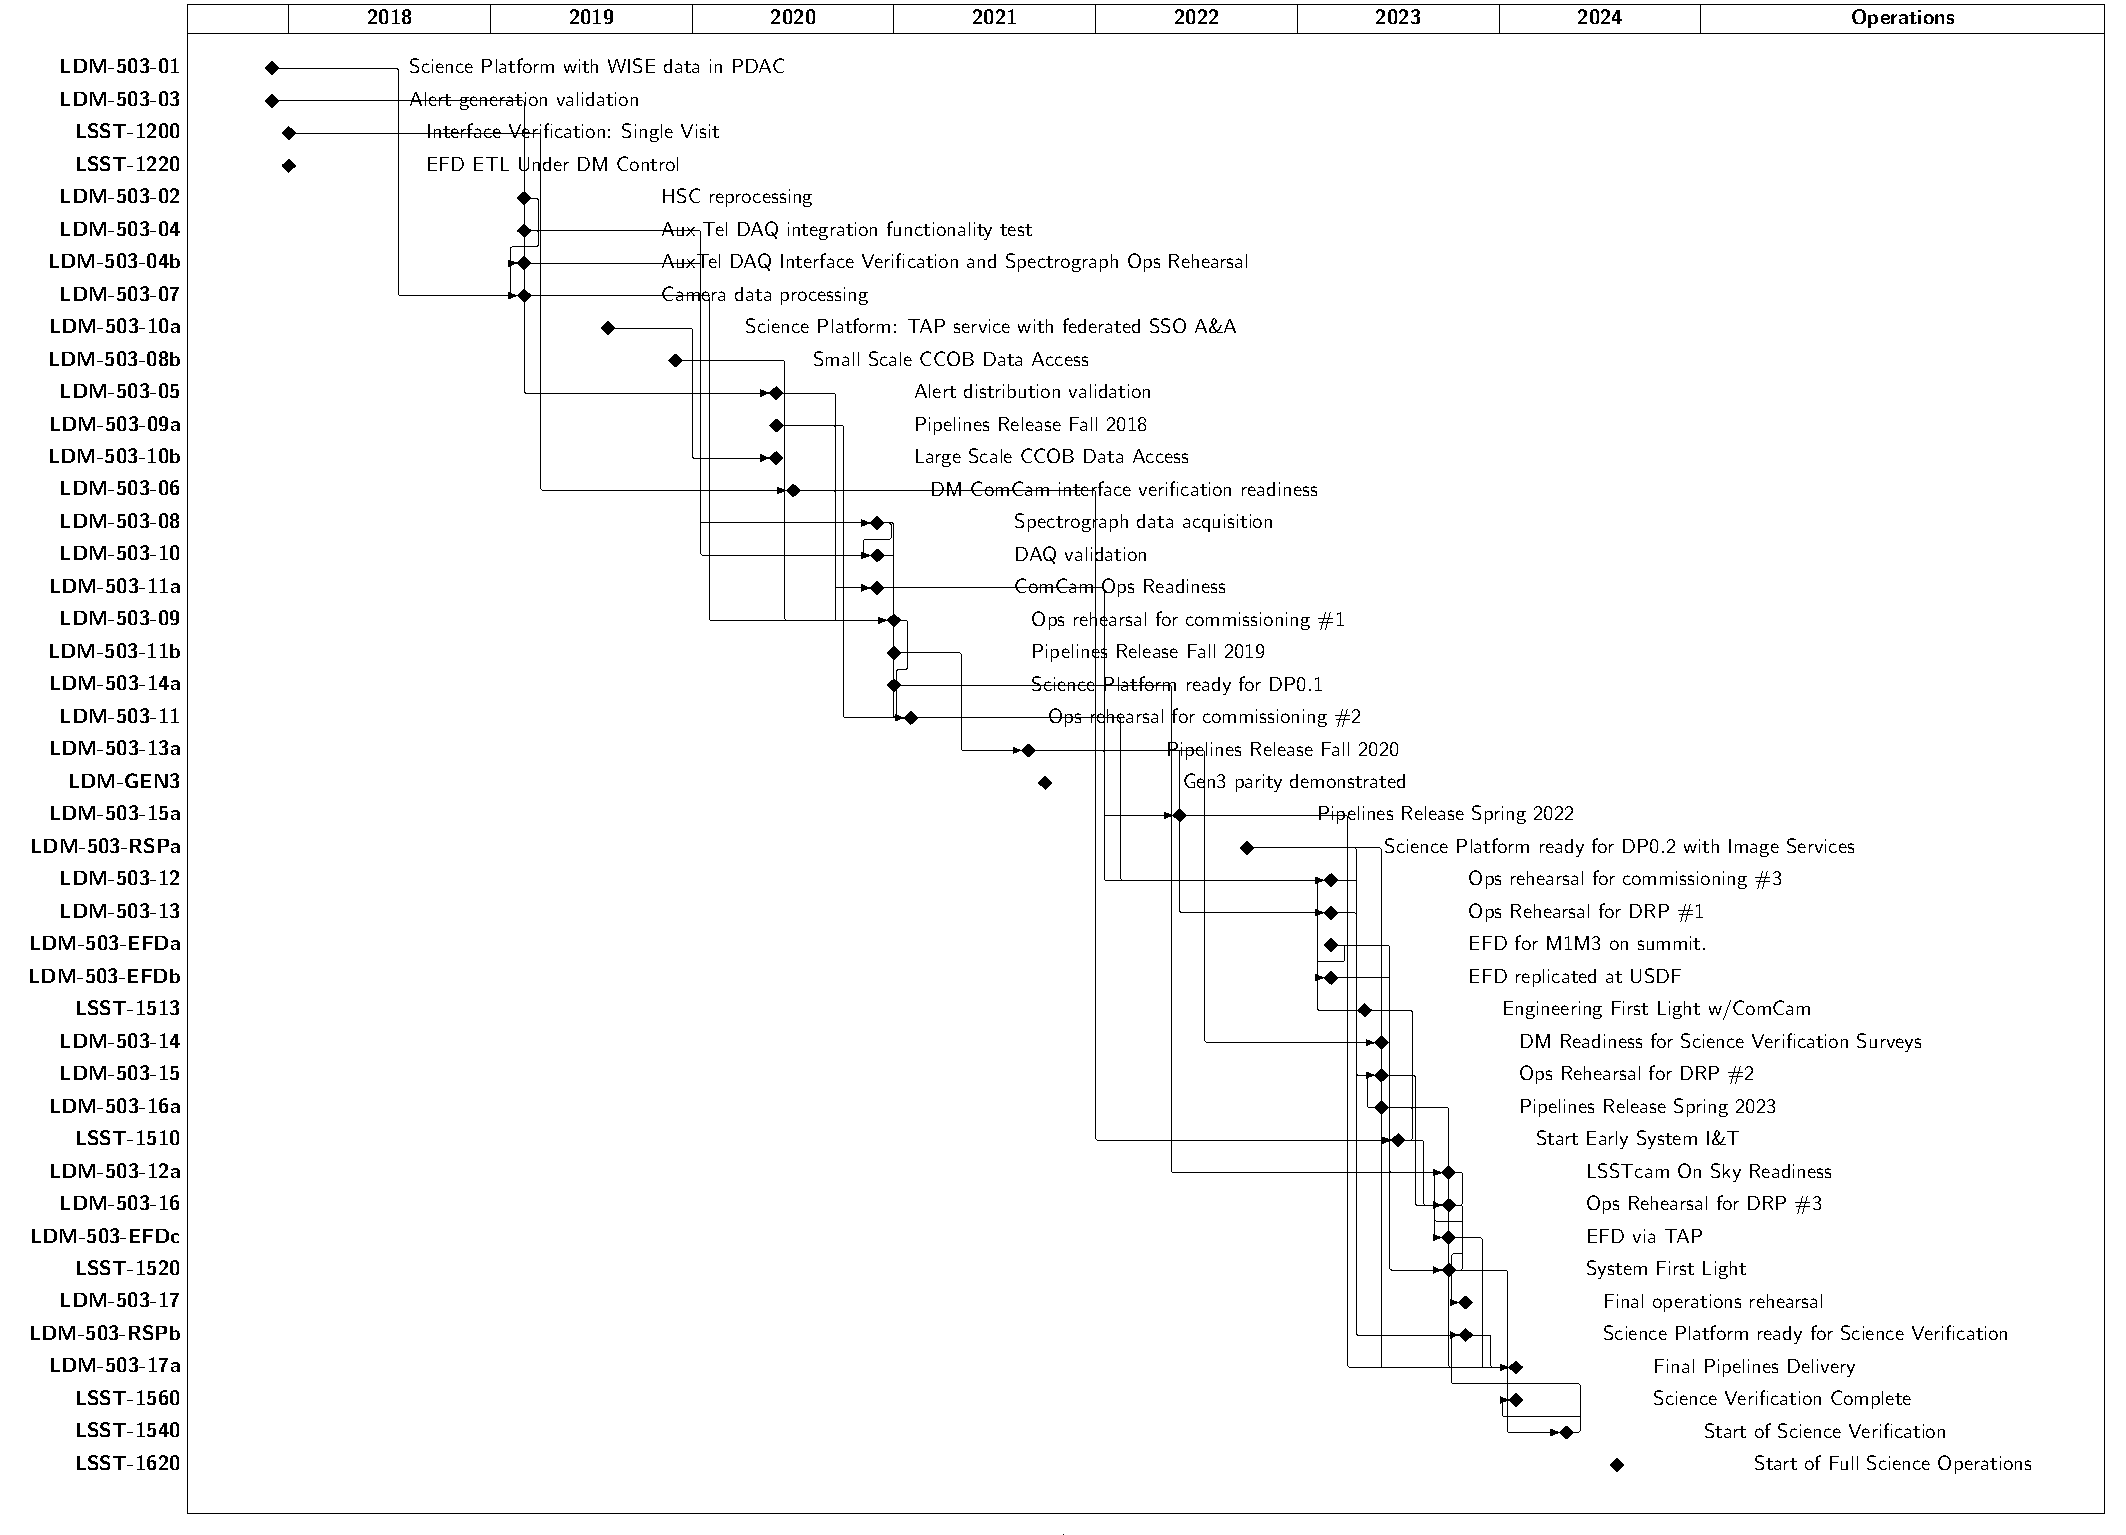
\includegraphics[width=1.1\textwidth]{gantt}
		 \caption{DM major milestones---designated as LDM-503-\textit{x}---in
         the Rubin schedule. These milestones are defined at level 2 according
         to the scheme described in \secref{sect:plan}. Status in \citeds{DMTN-158}}
         \label{fig:schedule}
 \end{figure}

\subsection{Work breakdown structure}\label{sect:WBS}

While the original DM WBS is laid out in \citeds{LPM-43} with definitions provided in \citeds{LPM-44},
the new WBS is currently described in \appref{sec:wbslist}, which is expected to replace the contents of LPM-43 upon approval by the Rubin CCB.

The WBS provides a hierarchical index of all hardware, software, services, and other deliverables which are required to complete the Rubin Project.
It consists of alphanumeric strings separated by periods.
The first component is always “1”, referring to the Rubin Construction Project.
``02C'' in the second component corresponds to Data Management Construction.
Subdivisions thereof are indicated by further digits.
These subdivisions correspond to teams within the DM project.
The top level WBS elements are mapped to the lead institutes in \tabref{tab:wbs}; the lead institutions roles are outlined in \secref{sect:leadtutes}.
The various groups involved in the WBS are briefly described in \secref{sect:groups}.

\begin{table}
\caption{DM top level Work Breakdown Structure \label{tab:wbs}}
\begin{center}
\begin{tabular}[htb]{|l|l|l|} \hline
\textbf{WBS}  &  \textbf{Description}   &  \textbf{Lead Institution}\\ \hline
1.02C.01& System Management                         &  Rubin Tucson \\ \hline
1.02C.02& Systems Engineering                       &  Rubin Tucson \\ \hline
1.02C.03& Alert Production                          &  University of Washington\\ \hline
1.02C.04& Data Release Production                   &  Princeton University\\ \hline
1.02C.05& Science User Interface and Tools          & IPAC\\ \hline
1.02C.06& Science Data Archive                      & SLAC\\ \hline
1.02C.07& LSST Data Facility                        & NCSA\\ \hline
1.02C.08& International Communications \& Base Site & Rubin Tucson \\ \hline
1.02C.09& System Level Testing \& Science Validation& Rubin Tucson \\ \hline
1.02C.10& Science Quality \& Reliability Engineering& Rubin Tucson \\ \hline
\end{tabular}
\end{center}
\end{table}

\subsection{Planning Process}\label{sect:plan}

Milestones have been defined to describe the major goals of the DM subsystem throughout the construction project.
Each milestone has a description, a due date, and a level.
Four levels are defined:

\begin{description}
\item[Level 1]{The most important milestones exposed at the NSF level.}
\item[Level 2]{Cross-subsystem milestones (for example, DM milestones that affect the Camera Subsystem).}
\item[Level 3]{Cross-team milestones within DM (for example, Middleware milestones that affect the DRP Team).}
\item[Level 4]{Internal milestones within a team.}
\end{description}

The major DM subsystem tests described in \secref{sect:schedule} are defined as level 2 milestones.
Teams plan their work towards each test by defining a series of level 3 milestones.
Teams may define level 4 milestones for their own use.

Resources to achieve the milestones throughout the duration of construction have been allocated by means of \textit{planning packages} loaded into the PMCS.
Each top level WBS within DM (per \tabref{tab:wbs}) is divided into some tens of planning packages, each of which addresses some part of the DM baseline design with a clearly defined scope, deliverable, resource cost, and end date.

As the due date for work approaches, the actions required to complete each planning package---and hence meet the associated milestones---must be defined in detail.
The DM team divides the year into two six month long \textit{cycles}, running from November through May (the ``spring cycle'') and from June through October (the ``fall cycle'').
At the start of each cycle, the DM Leadership Team (\secref{sect:dmlt}) agrees on the detailed plan of work for the cycle, and this is loaded in to Jira as a series of ``epics'', corresponding to projects of a few person-months duration, each with defined start and end dates and resource loading.
The DM team records work and tracks progress against epics using Jira; the Project Controller (\secref{role:pcon}) arranges for this information to be ingested to and made available within the PMCS.
When epics are closed the T/CAM should ensure the deliverables are mentioned/linked in the associated comments in Jira. The DMPM shall verify all closed epics have the defined deliverables associated with them.

This process is described in detail in \citeds{DMTN-020}.

All milestones status and tracking is provided monthly in \citeds{DMTN-158}.
